\chapter{Verfahren}
Das Verfahren besteht grundsätzlich aus 3 Schritten.
\section{Oclussionmap}
Zu erst wir eine Oclussionmap gerendert.
Diese stellt den Einflussbereich des Lichtes dar.\ref{o_1}
\begin{figure}
	\centering
	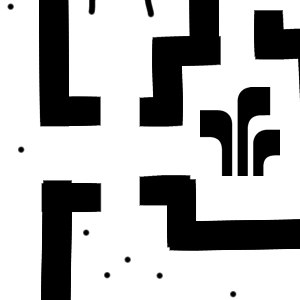
\includegraphics{images/oclusion.png}
	\caption{Oclussionmap}
	\label{o_1}
\end{figure}

\section{Sample Distance}
Anschließend wird das Oclusion Bild mit polarcoordinaten gesampled.
\begin{figure}
	\centering
	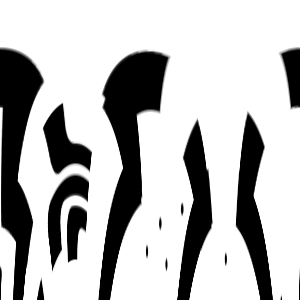
\includegraphics{images/oclusion_polar_2.png}
	\caption{Oclussionmap in polar Koordinaten}
	\label{o_2}
\end{figure}
Danach speichern wir die gesampelte minimal Distanz in einer 1D Textur.
\begin{figure}
	\centering
	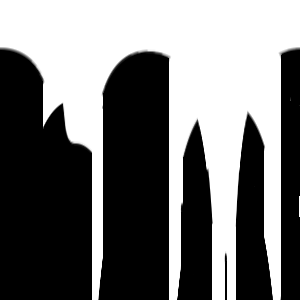
\includegraphics{images/shadow_polar_2.png}
	\caption{Symbolische Shadowmap in polar Koordinaten}
	\label{o_3}
\end{figure}
Als 1D Texture sieht das dann wie in Abbildung \ref{o_4} aus.
\begin{figure}
	\centering
	
\includegraphics{images/1DTexture.png}
	\caption{Gesampelte Distanzdaten.}
	\label{o_4}
\end{figure}